\section{Архитектура библиотеки}

\subsection{Структура}

Архитектура библиотеки представлена на рис.~\ref{fig:cubool_architecture}.
Структура библиотеки и ее конечначная функциональность в основном продиктованы следующими высокоуровневыми требованиями, которые продиктованы как конечными вычислительными задачами на GPGPU, так и наличием существующей инфраструктуры для осуществления экспериментов~\cite{net:cfpq_py_algo}.

\begin{itemize}
    \item Поддержка вычислений на Cuda-девайсе.
    \item Поддержка вычислений на CPU.
    \item C-совместимое API для работы с библиотекой.
    \item Python-пакет для работы с примитивами и операциями библиотеки в управляемой высокоуровневой стреде языка Python.
    \item Поддержка логирования, функций для отладки и протопирования конечных пользовательских алгоритмов.
\end{itemize}

\begin{figure}[h]
    \centering
    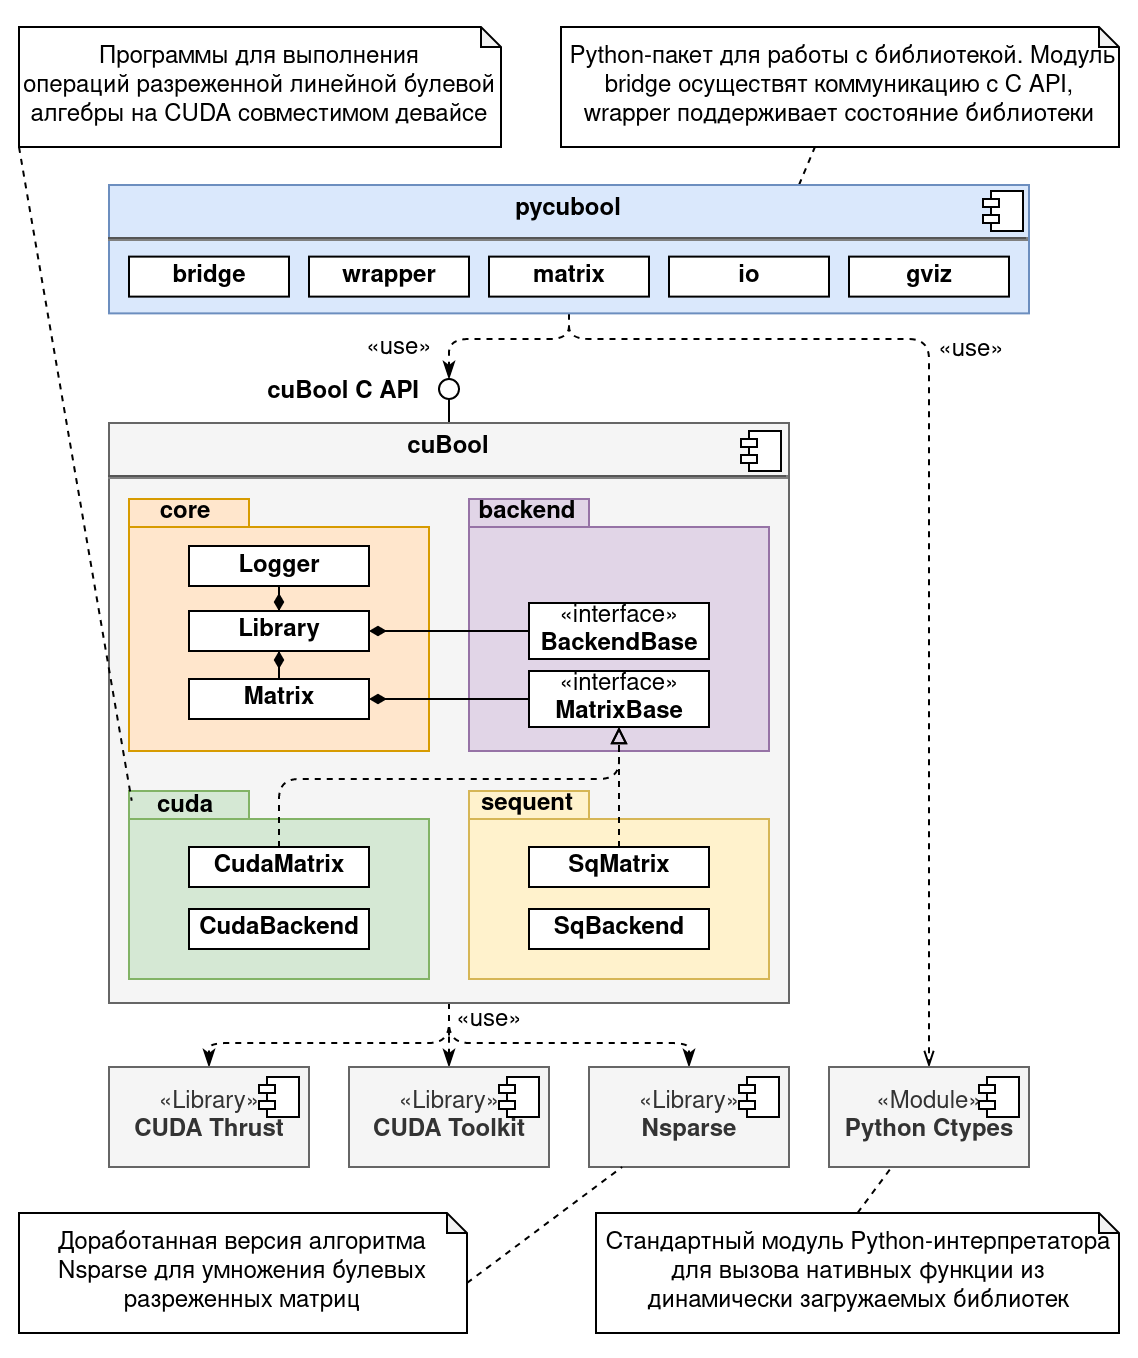
\includegraphics[width=0.8\textwidth]{images/library_architecture.png}
    \caption{Архитектура разработанной библиотеки}
    \label{fig:cubool_architecture}
\end{figure}

\subsection*{Core}

Класс \textbf{Library} поддерживает глобальное состояние библиотеки, осуществляет конфигурацию и инициализацию, выбор конкретного вычислительного бэкенда, первичную валидацию вызовов функций и входных данных пользователя, 
а также осуществляет хранение всех созданых объектов. 

Класс \textbf{Matrix} является proxy-классом, который осуществяет доступ к операциям конкретного вычислительного бэкенда, которой был выбран пользователем на этапе инициализации всей библиотеки.
Данный подход позволяет не только динамически выбирать платформу вычислений, 
но также позволяет осуществлять дополнительную обработку ошибок, 
а также поддерживать дополнительные операции над матрицами.

Класс \textbf{Logger} осуществляет логгирование в выбранный пользователем текстовый файл в процессе использования функций библиотеки, а также позволяет профилировать операций и также сохранять время их выполенения в текстовом виде.

\subsection*{Backend}

Интерфейс \textbf{MatrixBase} предоставляет набор основных функций и операций, которые каждый вычислительный бэкенд должен реализовывать для того, чтобы эти матрицы можно было использовать в \textbf{Core} непосредственно для вычислений.

Интерфейс \textbf{BackendBase} описывает базовый контракт, которой должен предоставлять вычислительный бэкенд. Данный интерфейс включает в себя функции для создания и удаления матриц, спефичных для этого буэкенда, а также функции для корректной инициализации и завершения работы данного бэкенда.

\subsection*{Cuda}

Класс \textbf{CudaMatrix} реализует интерфейс \textbf{MatrixBase} и предоставляет операции, для работы с матрицами и осуществления вычислений на Cuda-девайсе. \textbf{CudaMatrix} поддерживает данные матрицы (не нулевые элементы) в видео-памяти, и использует Cuda \textit{kernels} для осуществления вычислений на GPU. \textit{Kernels} хранятся в виде функций вместе с исходным кодом модуля.

Данный вычислительный бэкенл выбирается по умолчанию, если в компьтере пользователся имеется Cuda-девайс.
Однако пользователь может в таком случае все равно может выбрать \textbf{Sequent} вычисления. 

\subsection*{Sequent}

Предоставляет реализацию класса матрицы и операций над ней для вычислений на CPU. Все вычислений осуществляются последовательно, в однопоточном режиме, не требуют дополнительных библиотек или компонентов.

Данных вычислительный бэкенд используется по умолчанию на устройствах без Cuda-девайса. Данный подход позволит использовать библиотеку всем пользователям без исключения. Также данный подход может быть удобен для прототипирования алгоритмов на локальном компьютере, чтобы позже запустить вычисления на высокопроизводительном сервере с поддержкой Cuda.

\subsection*{Pycubool}

Python-пакет предоставляет доступ к примитивам и операциям библиотеки в языковой среде Python.
Модуль \textbf{matrix} предоставляет доступ к классу матрицы и основным операциям, дотсупным в C API.
Модуль \textbf{bridge} осуществляет коммуникацию с библиотекой через механизмы вызова нативных методов. Модуль \textbf{wrapper} поддерживает глобальное состояние библиотеки в во время работы Python-интерпретатора. Модули \textit{io} и \textbf{gviz} предоставляют доступ к операциям ввода/вывода данных, позволяют загружать или сохранять матрциы в виде текстовых на диск, а также экспортировать набор матриц в виде графа в формате GraphViz, что может быть полезно для отладки алгоритмов.

\subsection{Последовательнось обработки операций}

На рис.~\ref{fig:cubool_sequence} представлена последовательность обработки вычислительной операции над матрицей (матрицами) на Cuda-девайсе. 

Пользовательский Python-код инициирует выполнение операции над мамтрицей или несколькими матрицами внутри инфраструктуры Python. Этот вызов обрабатывает \textbf{pycubool}-пакет, который осуществляет первичную базовую валидацию аргументом, осуществляет их запаковку и передачу в нативную функцию \textbf{cuBool C API}. На стороне реализации данного интерфейса, полученные аргументы приводятся к требуемому типу и передаются далее в модуль \textbf{Core}, который поддерживает состояние библиотеки, осуществяет валидацию аргументов, а также определяет допустимость выполнения операции. Далее вызов передается непосредственно вычислительному бэкенду \textbf{Cuda}, который осуществляет подготовку и непосредственный запуск вычислений на сороне \textbf{Nvidia GPU}. 

Когда вычисление завершается, \textbf{Cuda}-бэкенд обновляет состояние матриц в соответсвии с полученными результами. Модуль \textbf{Core} осуществяет финальное логирование операции, а также сохраняет временные показатели выполнения вычислений в файл (опционально), и возвращает в качестве результата выполнения статус операции, либо возможное исклбчение, которое могло возникнуть на этапе обработки запроса вычислений. \textbf{cuBool C API} осуществяет финальную обработку исключения (если таковое возникло), и возвращет вызываещему числовой идентефикатор статуса операции. 

В результате выполнения операции \textbf{pucubool} уведомляет пользователя о потенциально возникших ошибках и возвращает управление из вызываемой функции. Обновленное состояние библиотеки находится в \textbf{Core}, а состояние матриц после выполнения операций хранится на стороне \textbf{Cuda}-бэкенда. 

\begin{figure}[h]
    \centering
    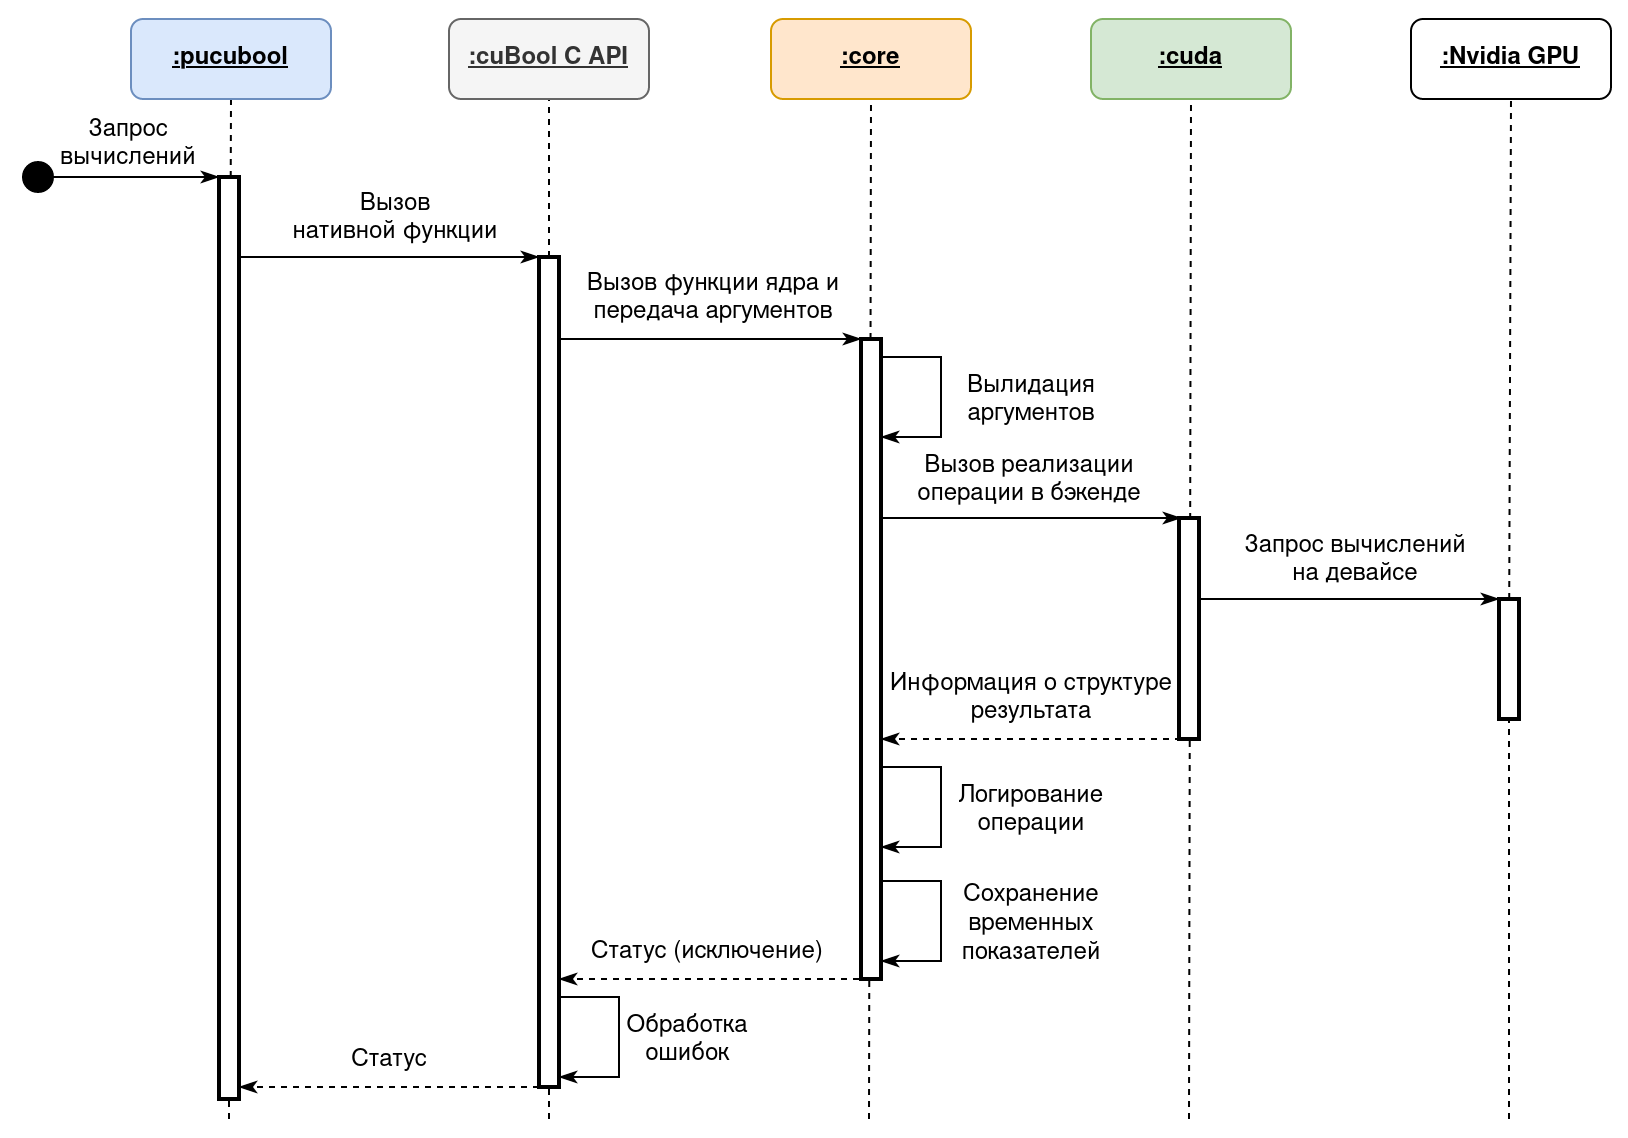
\includegraphics[width=0.8\textwidth]{images/library_sequence_use.png}
    \caption{Последовательность обработки вызова вычислительной матричной операции на Nvidia GPU}
    \label{fig:cubool_sequence}
\end{figure}


